\documentclass[conference]{IEEEtran}
\IEEEoverridecommandlockouts
% The preceding line is only needed to identify funding in the first footnote. If that is unneeded, please comment it out.
%Template version as of 6/27/2024

\usepackage{cite}
\usepackage{amsmath,amssymb,amsfonts}
\usepackage{algorithmic}
\usepackage{graphicx}
\usepackage{textcomp}
\usepackage{xcolor}

\usepackage{float} 
\usepackage{placeins}

\usepackage{colortbl}  % Required for \rowcolor
\usepackage{xcolor}    % Provides additional color definitions

% Digunakan untuk menampilkan pustaka.
\usepackage[square,comma,numbers,sort&compress]{natbib}

% Mengubah format ukuran teks pada natbib.
\renewcommand{\bibfont}{\normalfont\footnotesize}

% Digunakan untuk menyeimbangkan bagian akhir dokumen dengan dua kolom.
\usepackage{balance}

\def\BibTeX{{\rm B\kern-.05em{\sc i\kern-.025em b}\kern-.08em
    T\kern-.1667em\lower.7ex\hbox{E}\kern-.125emX}}
\begin{document}


% \title{AUTONOMOUS VEHICLE NAVIGATION SYSTEM USING MACHINE LEARNING AND GRAPH BASED SLAM
% }
\title{AUTONOMOUS VEHICLE NAVIGATION FOR HEAVY INDUSTRIAL TRANSPORT WITH HIGH ACCURACY AND PRECISION POSE USING GRAPH-BASED SLAM AND REAL-TIME MACHINE LEARNING}

\author{\IEEEauthorblockN{Azzam Wildan Maulana}
\IEEEauthorblockA{\textit{Departemen of Electrical Engineering} \\
\textit{Faculty of Intelligent Electrical and Informatics Technolog} \\
\textit{Sepuluh Nopember Institute of Technology}\\
Surabaya, Indonesia \\
azzamwildan462@gmail.com}
\and

\IEEEauthorblockN{Rudy Dikairono}
\IEEEauthorblockA{Department of Electrical Engineering\\
Faculty of Intelligent Electrical and Informatics Technology\\
Institut Teknologi Sepuluh Nopember\\
Surabaya, Indonesia 60111\\
rudydikairono@its.ac.id}
\and

\IEEEauthorblockN{Ahmad Zaini}
\IEEEauthorblockA{Department of Computer Engineering\\
Faculty of Intelligent Electrical and Informatics Technology\\
Institut Teknologi Sepuluh Nopember\\
Surabaya, Indonesia 60111\\
zaini@its.ac.id}
\and

\IEEEauthorblockN{Mauridhi Hery Purnomo}
\IEEEauthorblockA{\textit{Departemen of Computer Engineering} \\
\textit{Faculty of Intelligent Electrical and Informatics Technolog} \\
\textit{Sepuluh Nopember Institute of Technology}\\
Surabaya, Indonesia \\
hery@ee.its.ac.id}
\and
}

\maketitle

\begin{abstract}
	Indonesia Smelting Technology (IST) is an industry below Toyota Tsusho Corp that focuses on producing aluminum liquid. The melted aluminum liquid will be used by CMWI (Central Motor Wheel Indonesia) to make the wheel rims. IST has a vision to become a smart factory that utilizes the latest technology in its operations. One of the technologies that can be implemented is autonomous vehicles, which can transport a dangereous aluminum liquid (molten) from IST to CMW. The total weight of the molten aluminum liquid is around 1.8 tons, and the total weight that the vehicle need to carry is 4.8 tons. Previously, IST has used a small train with a rail to transport the molten aluminum liquid, but this method has several limitations, such as the need for a rail infrastructure that very expensive and the limited flexibility of the vehicle. So, IST wants to implement an autonomous vehicle that can transport the molten aluminum liquid without the need for a rail infrastructure. The autonomous vehicle will be equipped with a navigation system that can detect the lane and obstacles, and can navigate autonomously to the destination. The navigation system will use a combination of machine learning and graph-based SLAM (Simultaneous Localization and Mapping) to achieve this goal. The machine learning algorithm will be used to detect the lane and obstacles, while the graph-based SLAM will be used to estimate the pose of the vehicle and create a map of the environment. The result of this research is a cm level error (below 1 cm) in robot pose estimation and a lightweight machine learning model that can run only on CPU with below 10 ms inference time.
\end{abstract}

\begin{IEEEkeywords}
	autonomous vehicle, navigation system, machine learning, graph-based SLAM, lane detection
\end{IEEEkeywords}

\section{Background}
Indonesia Smelting Technology (IST) is an industry below Toyota Tsusho Corp that focuses on producing aluminum liquid. The environment in IST is very dangereous because of the molten aluminum liquid that has a temperature of around 700 degrees Celsius. The production goes in 24 hours a day. The production team divided into three shifts. The research from \cite{ref_sleep} said that there will be more sleepy workers in the night shift. The sleepy workers will be more prone to accidents even if doing micro sleep for 1-2 seconds. The industry (IST) said there were much accidents in the night shift, such as workers grazed to nearby pole or wall and the spilled of the molten aluminum liquid that been carried by the workers. By many accidents, the industry (IST) wants to implement an autonomous vehicle that can transport the molten aluminum liquid from IST to CMWI (Central Motor Wheel Indonesia). 

\par    
For the vehicle itself, there is a Towing that previously operated by the workers. The goal of my team is to modify that Towing to be fully autonomous. To design the autonomous vehicle for the harsh environment, the vehicle need to be robust on its hardware and software. The hardware need to be always on and can handle the harsh environment such is high temperature, high conductive dust level, and high vibration. In the other hand, the software need to be low power, low latency, but has high accuracy.

\par    
For the high accuracy, we choose the Graph Based SLAM (Simultaneous Localization and Mapping) as the main algorithm to estimate the pose of the vehicle. There is a framework to do that called RTAB-Map. The RTAB-Map is a graph-based SLAM that can handle large scale environment and can run on low power hardware. The RTAB-Map can also handle the loop closure detection, which is very important for the autonomous vehicle to navigate in the environment. The RTAB-Map can also handle the dynamic environment, which is very important for the autonomous vehicle to navigate in the environment. The RTAB-Map can also handle the large scale environment, which is very important for the autonomous vehicle to navigate in the environment \cite{ref_rtabmap}.  

\par    
For the low power and low latency of lane detection, we modify the Fast-SCNN model \cite{ref_fast_scnn} to be more lightweight and can run on CPU. Fast-SCNN is a semantic segmentation model that use a skip connection inside its network architecture to get the spatial information from the input image. But the Fast-SCNN model is still too heavy to run on CPU, so we modify the model to be more lightweight.  

% =========================================================================================================

\section{Methodology}
The methodology of this research is divided into four parts. First part is the pose estimation using graph-based SLAM, the third part is the lane detection using machine learning, and the last part is the integration of the navigation system and safety system. 

\subsection{Pose Estimation using Graph-Based SLAM}
\begin{figure}[H]
	\centering
	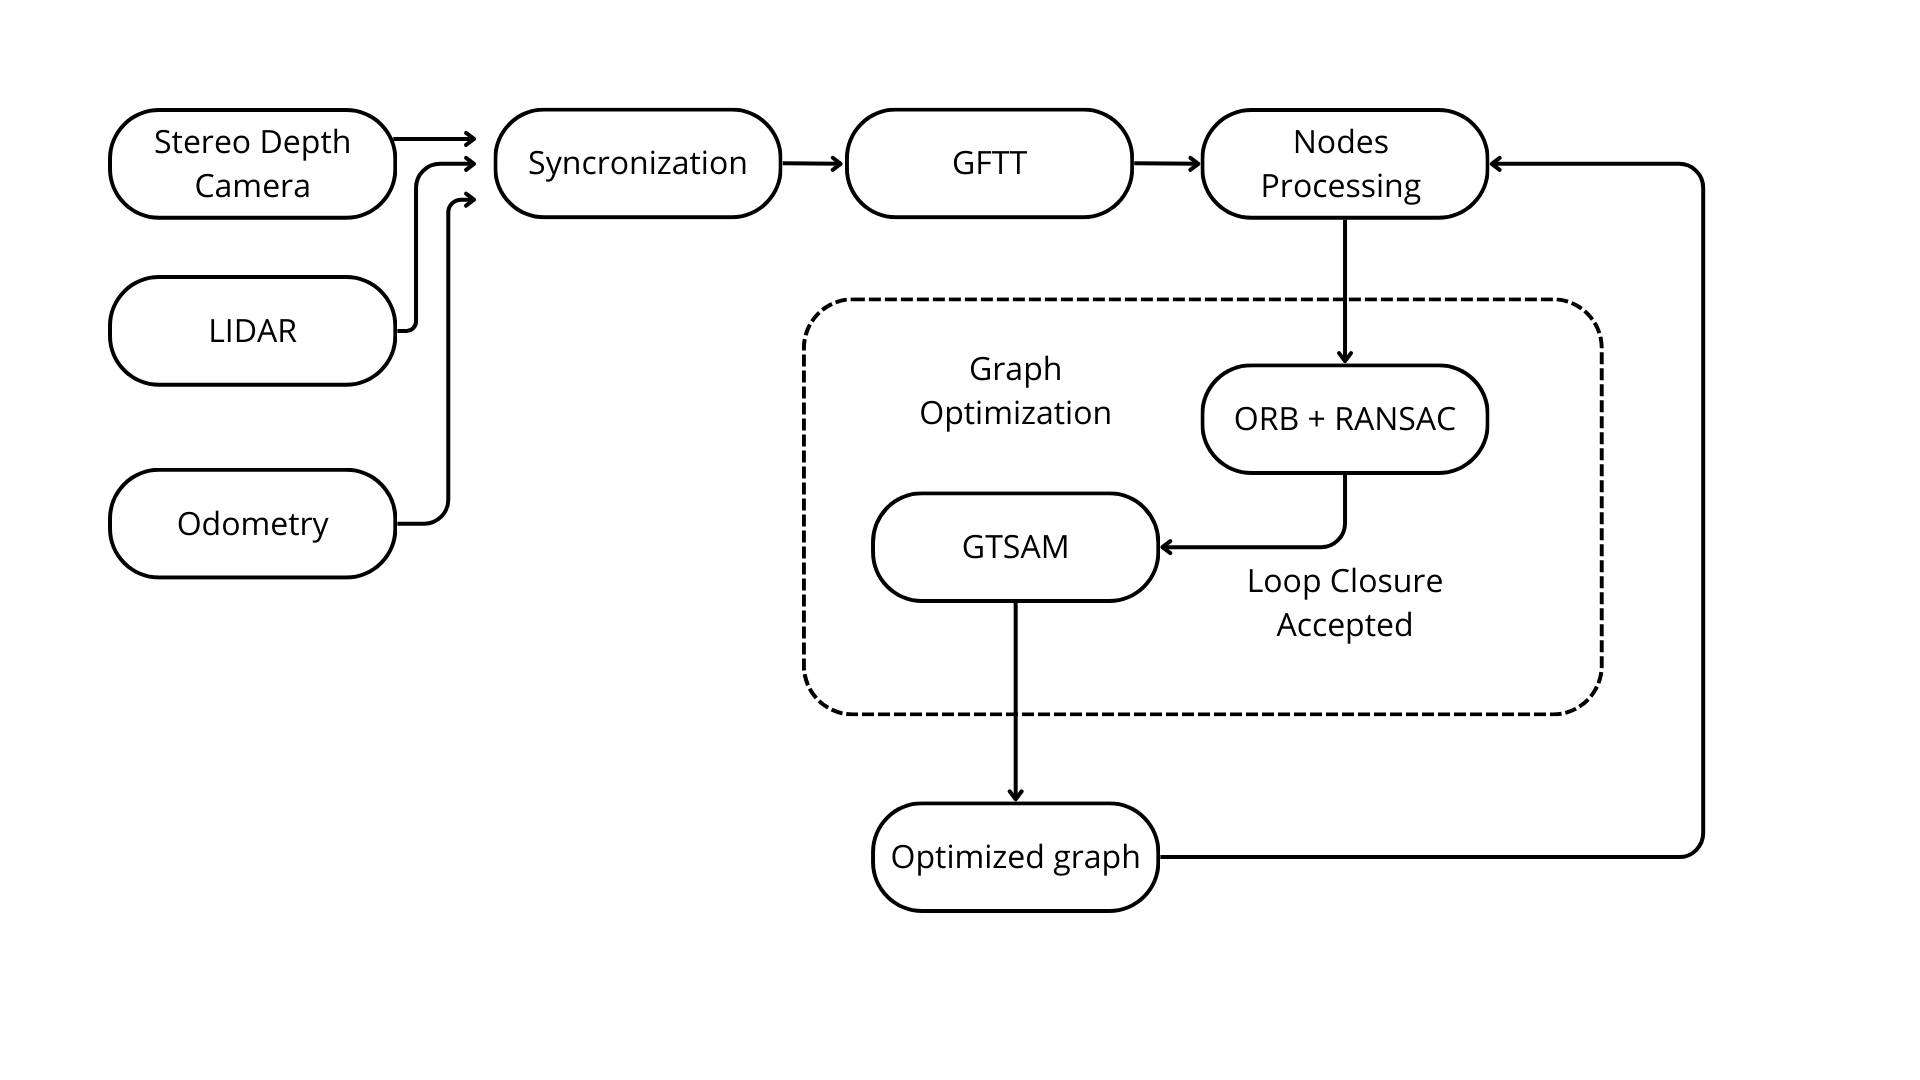
\includegraphics[width=\linewidth]{../konten/nav_map2.png}
	\caption{Block Diagram of Graph Based SLAM in Mapping Mode}
	\label{fig:slam_system}
\end{figure} 

From the figure \ref{fig:slam_system}, we can see that the navigation system used on Autonomous Towing. The first step is calculate the odometry from the Towing. The odometry is calculated from the encoder speed and IMU data. By using inverse kinematics from encoder speed and IMU data, we can calculate the speed of Towing. 

\begin{equation}
	v\theta = \frac{\text{current\_IMUyaw} - \text{previous\_IMUyaw}}{\Delta t}
	\label{eq:vtheta}
\end{equation}

Where \(\Delta t\) is the time difference between the current and previous IMU data. The \(\text{current\_IMUyaw}\) and \(\text{previous\_IMUyaw}\) are the yaw angle of the IMU in radians. \(v\theta\) is the angular velocity of the Towing in radians per second in yaw component.

\begin{equation}
	v_x = \frac{\text{encoder\_speed} \cdot \cos(\theta) \cdot \text{encoder\_to\_meter}}{\Delta t}
	\label{eq:vx}
\end{equation}

Where \(\text{encoder\_speed}\) is the speed of the Towing from the encoder in RPM, \(\theta\) is the yaw angle of the Towing in radians, and \(\text{encoder\_to\_meter}\) is the conversion factor from encoder speed to meter per second. The \(\Delta t\) is the time difference between the current and previous encoder data. \(v_x\) is the linear velocity of the Towing in meter per second in x component.

\begin{equation}
	v_y = \frac{\text{encoder\_speed} \cdot \sin(\theta) \cdot \text{encoder\_to\_meter}}{\Delta t}
	\label{eq:vy}
\end{equation}

Where \(\text{encoder\_speed}\) is the speed of the Towing from the encoder in RPM, \(\theta\) is the yaw angle of the Towing in radians, and \(\text{encoder\_to\_meter}\) is the conversion factor from encoder speed to meter per second. The \(\Delta t\) is the time difference between the current and previous encoder data. \(v_y\) is the linear velocity of the Towing in meter per second in y component.

\par    
The second step is data acquisition and data syncronization. This can be done by using a routine timer that grab the data with same stamped time. The technique called approximate time syncronization with the delay tolerance about 10 ms. 

\par    
The third step is Nodes processing, which is the process of creating a node from the data acquired. There is a bit different in Nodes processing between Mapping mode and localization mode. In mapping mode, The nodes will always be updated. In localization mode, the nodes will not be updated. Each node in the graph contains: 
\begin{itemize}
	\item \textbf{Pose}: The pose of the Towing in the world frame that come from integration of odometry.
	\item \textbf{Optimized Pose}: The pose of the Towing after optimized.
	\item \textbf{Sensor Data}: The sensor data from the camera and lidars.
	\item \textbf{Timestamp}: The timestamp of the node.
	\item \textbf{Keypoint}: The result of the GFTT features. 
	\item \textbf{Weight}: Weight for graph optimization (GTSAM). 
\end{itemize}

\par    
Next step is ORB + RANSAC process, while the Towing has moved to map the area, the ORB process will find the matched keypoint from current synchronized camera data to all the saved node. After ORB found some matched keypoint, the next process is RANSAC filter. The RANSAC filter will filter the matched keypoint geometrically \cite{ref_orb_ransac}. The output of RANSAC filter is the inliers between two image. If the inliers is more than the mininimum thershold, the loop closure hypothesis will be added. Below is the result example of ORB + RANSAC. 
\begin{figure}[H]
	\centering
	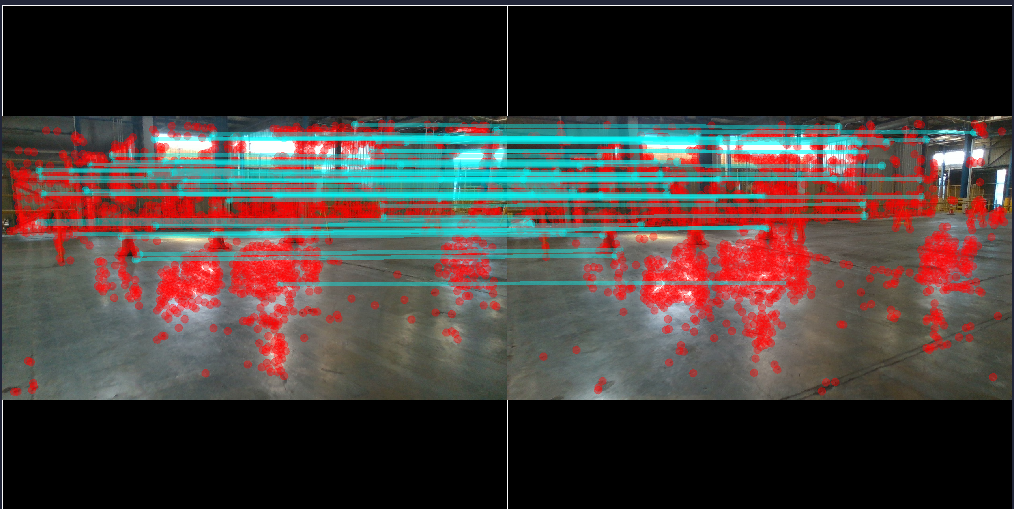
\includegraphics[width=\linewidth]{../konten/orb_ransac2.png}
	\caption{Result of ORB + RANSAC}
	\label{fig:orb_ransac}
\end{figure}
The figure \ref{fig:orb_ransac} shows the result of ORB + RANSAC process. The left image is the current synchronized camera data, and the right image is the saved node. The cyan lines are the matched keypoint between two images. The red points are the features detected by GFTT (Good Features to Track) algorithm \cite{ref_gftt}.
\par   
After loop closure hypothesis is added, the next step is to optimize the graph. The optimization process will use GTSAM library \cite{ref_gtsam} to optimize the graph. The optimization process will use the ICP as the constraint between the nodes. All the nodes link constraint calculated using ICP from the lidar laser scan. If the iterations for optimizing has reached the maximum iterations, the optimization process will stop and the minimum error will be noted. If the minimum error is below the threshold, the loop closure will be accepted and the graph will be updated. The optimized pose will be calculated for every node and updated for all nodes in the graph. The optimized pose will be used for the next localization process. Below is the example of the map that has been built with and without loop closure found. 

\begin{figure}[H]
	\centering
	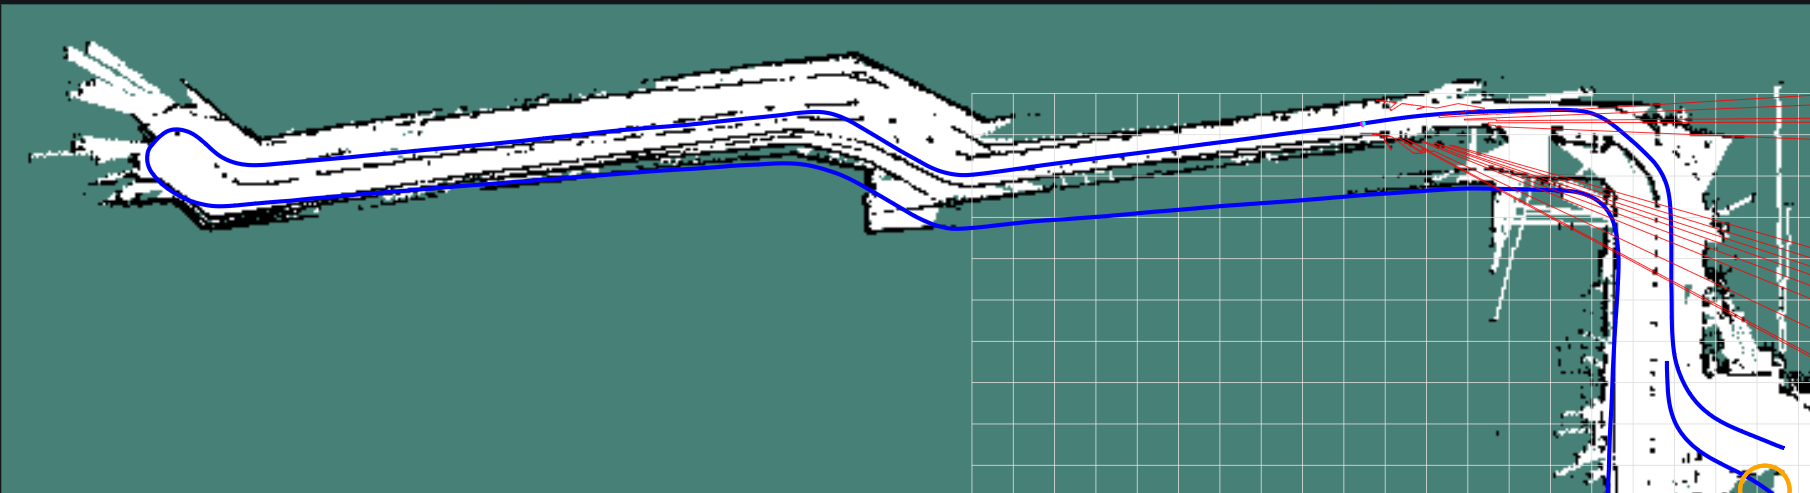
\includegraphics[width=\linewidth]{../konten/map_salah.png}
	\caption{Map of the area without loop closure found.}
	\label{fig:map}
\end{figure}

The figure \ref{fig:map} shows the map of the area with and without loop closure found. We can see that the map has not match the real world environment because of the drift odometry error. After loop closure has been found and all the graph were optimized, the map will be updated. Below is the example of the map that has been built with loop closure found.

\begin{figure}[H]
	\centering
	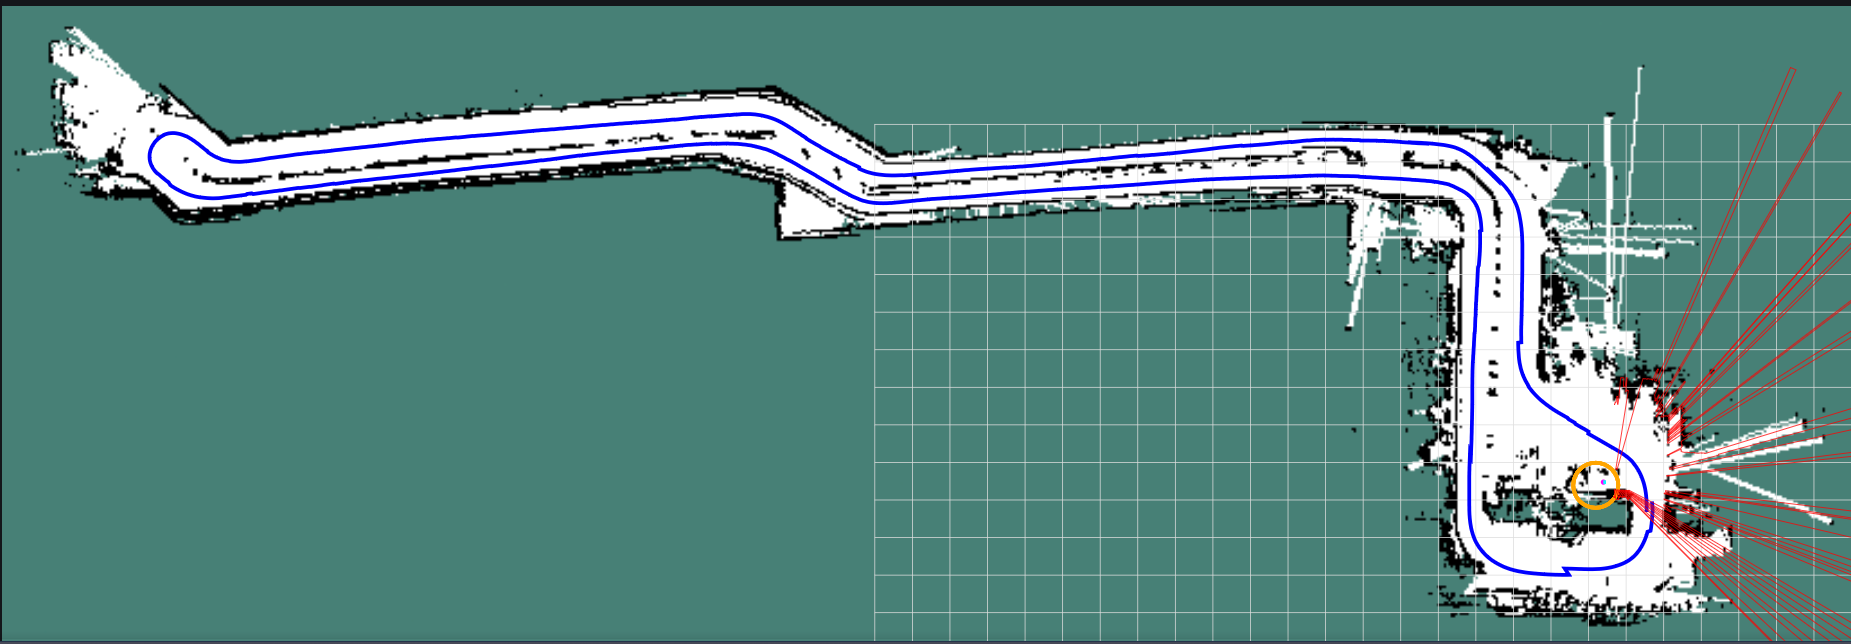
\includegraphics[width=\linewidth]{../konten/map_benar.png}
	\caption{Map of the area with loop closure found.}
	\label{fig:map_corrected}
\end{figure}

The figure \ref{fig:map_corrected} shows the map of the area with loop closure found. We can see that the map has been corrected and match the real world environment. The optimized pose will be used for the next localization process.

\begin{figure}[H]
	\centering
	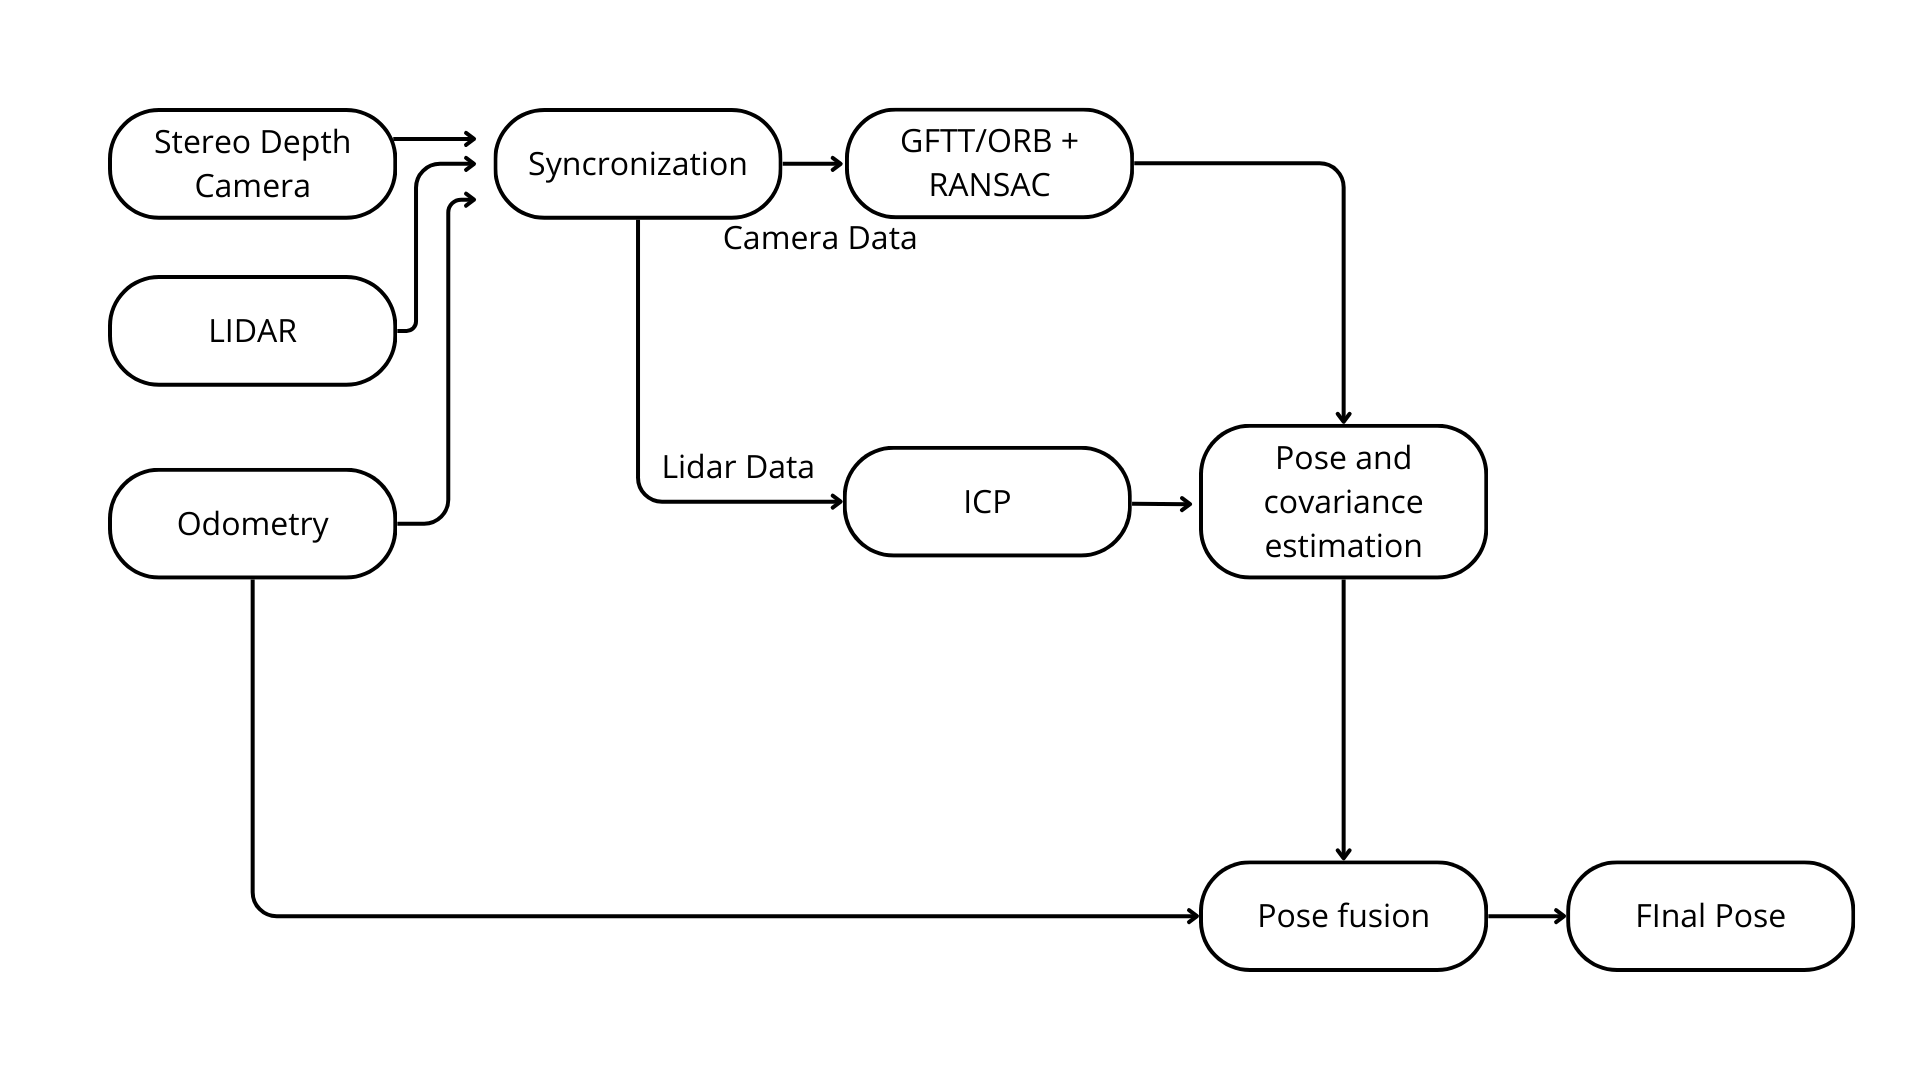
\includegraphics[width=\linewidth]{../konten/nav_loc2.png}
	\caption{Block Diagram of Graph Based SLAM in Localization Mode}
	\label{fig:slam_system_loc}
\end{figure} 

In the localization mode, the process is almost the same as in mapping mode. The difference is that the nodes will not be updated, and the optimized pose will be used for localization. The localization process will use the current synchronized camera data to find the matched keypoint to all the saved node. After ORB found some matched keypoint, the next process is RANSAC filter. The RANSAC filter will filter the matched keypoint geometrically. The output of RANSAC filter is the inliers between two image. If the inliers is more than the minimum threshold, the corrected pose and covariance will be calculated using ICP constraint. 

\par    
After the corrected pose and covariance is calculated, the next step is the pose fusion between corrected pose and covariance with the raw odometry pose and covariance. The raw odometry is coming from equation \ref{eq:vtheta}, \ref{eq:vx}, and \ref{eq:vy}. The pose fusion will use the Kalman Filter to fuse the corrected pose and covariance with the raw odometry pose and covariance. The output of the pose fusion is the final pose that will be used in navigation system.

\subsection{Lane Detection using Machine Learning}
\begin{figure}[H]
	\centering
	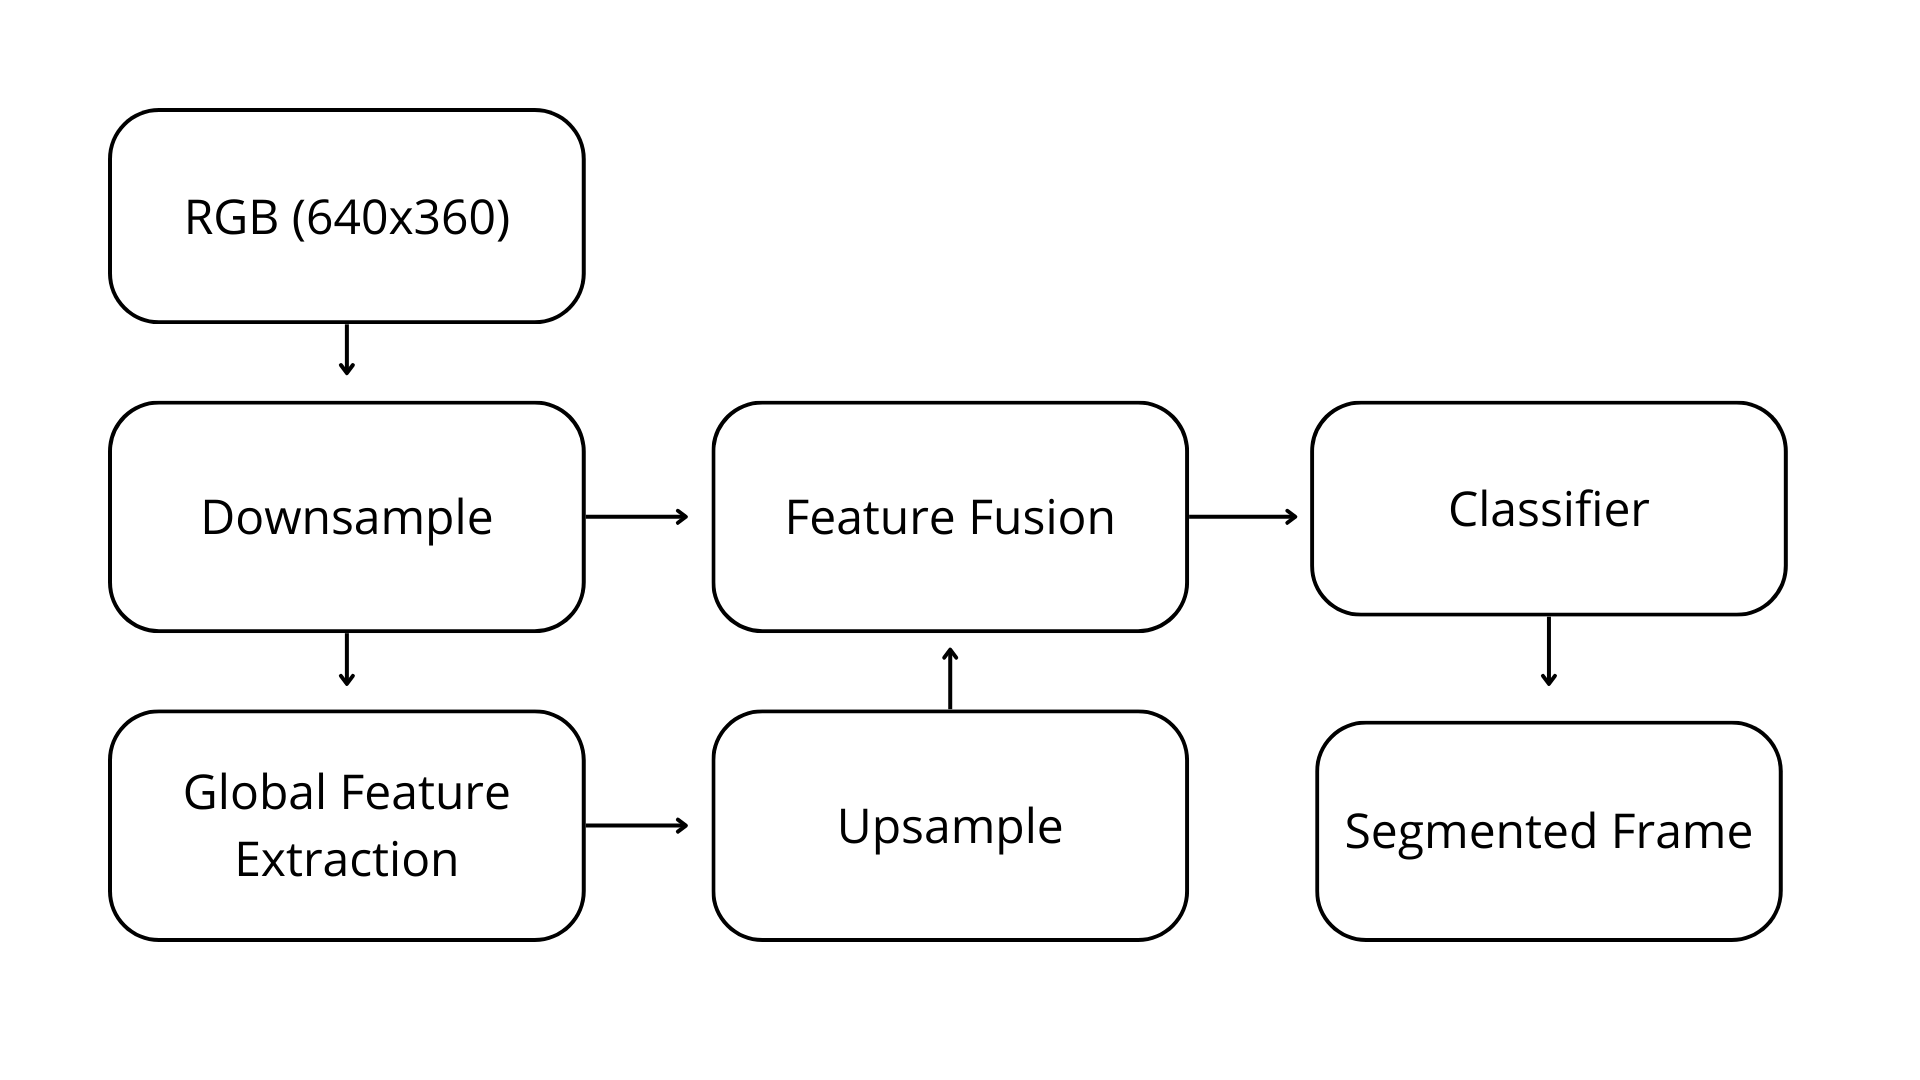
\includegraphics[width=\linewidth]{../konten/ml_sys.png}
	\caption{Block Diagram of the Machine Learning Architecture}
	\label{fig:ml_system}
\end{figure} 


From Figure \ref{fig:ml_system}, it is shown that the lane detection system on Autonomous Towing utilizes a machine learning architecture, specifically using Fast-SCNN \cite{ref_fast_scnn} as the core model. Our architecture differs in the convolution channels and pooling methods. The smaller convolution channels and the use of average pooling instead of pyramid pooling are intended to reduce computational load, making it suitable for real-time applications on Autonomous Towing.

\subsubsection{Downsampling} 
In this step, the image captured by the stereo depth camera, originally a 3-channel image, is converted to 16 channels. This is achieved via three successive 3x3 convolution layers with a stride of 2: first converting 3→8 channels, then 8→16, and finally 16→32 channels. The resulting image is then split into two paths: one goes to global feature extraction, the other to feature fusion. 

\subsubsection{Global Feature Extraction}
This stage performs a depthwise-separable convolution to extract features from the 32-channel image. This method is chosen for its computational efficiency. The result is a 48-channel image, which is passed on to the upsampling stage. 

\subsubsection{Upsampling}
This step performs pooling using average pooling, which is lighter and faster compared to the pyramid pooling used in the original Fast-SCNN. A convolution then produces a 64-channel output, which is passed to feature fusion.

\subsubsection{Feature Fusion}
Here, outputs from the downsampling (32 channel) and global feature extraction (64 channel) stages are merged into a 96-channel image. Before merging, image dimensions are matched using bilinear interpolation. The merged result is passed to the classification stage.

\subsubsection{Classification}
In this final stage, the 96-channel image undergoes classification using ReLU, producing a 1-channel image indicating road areas. This image then proceeds to post processing.

\subsection{Integration of Navigation System and Safety System}
\begin{figure}[H]
	\centering
	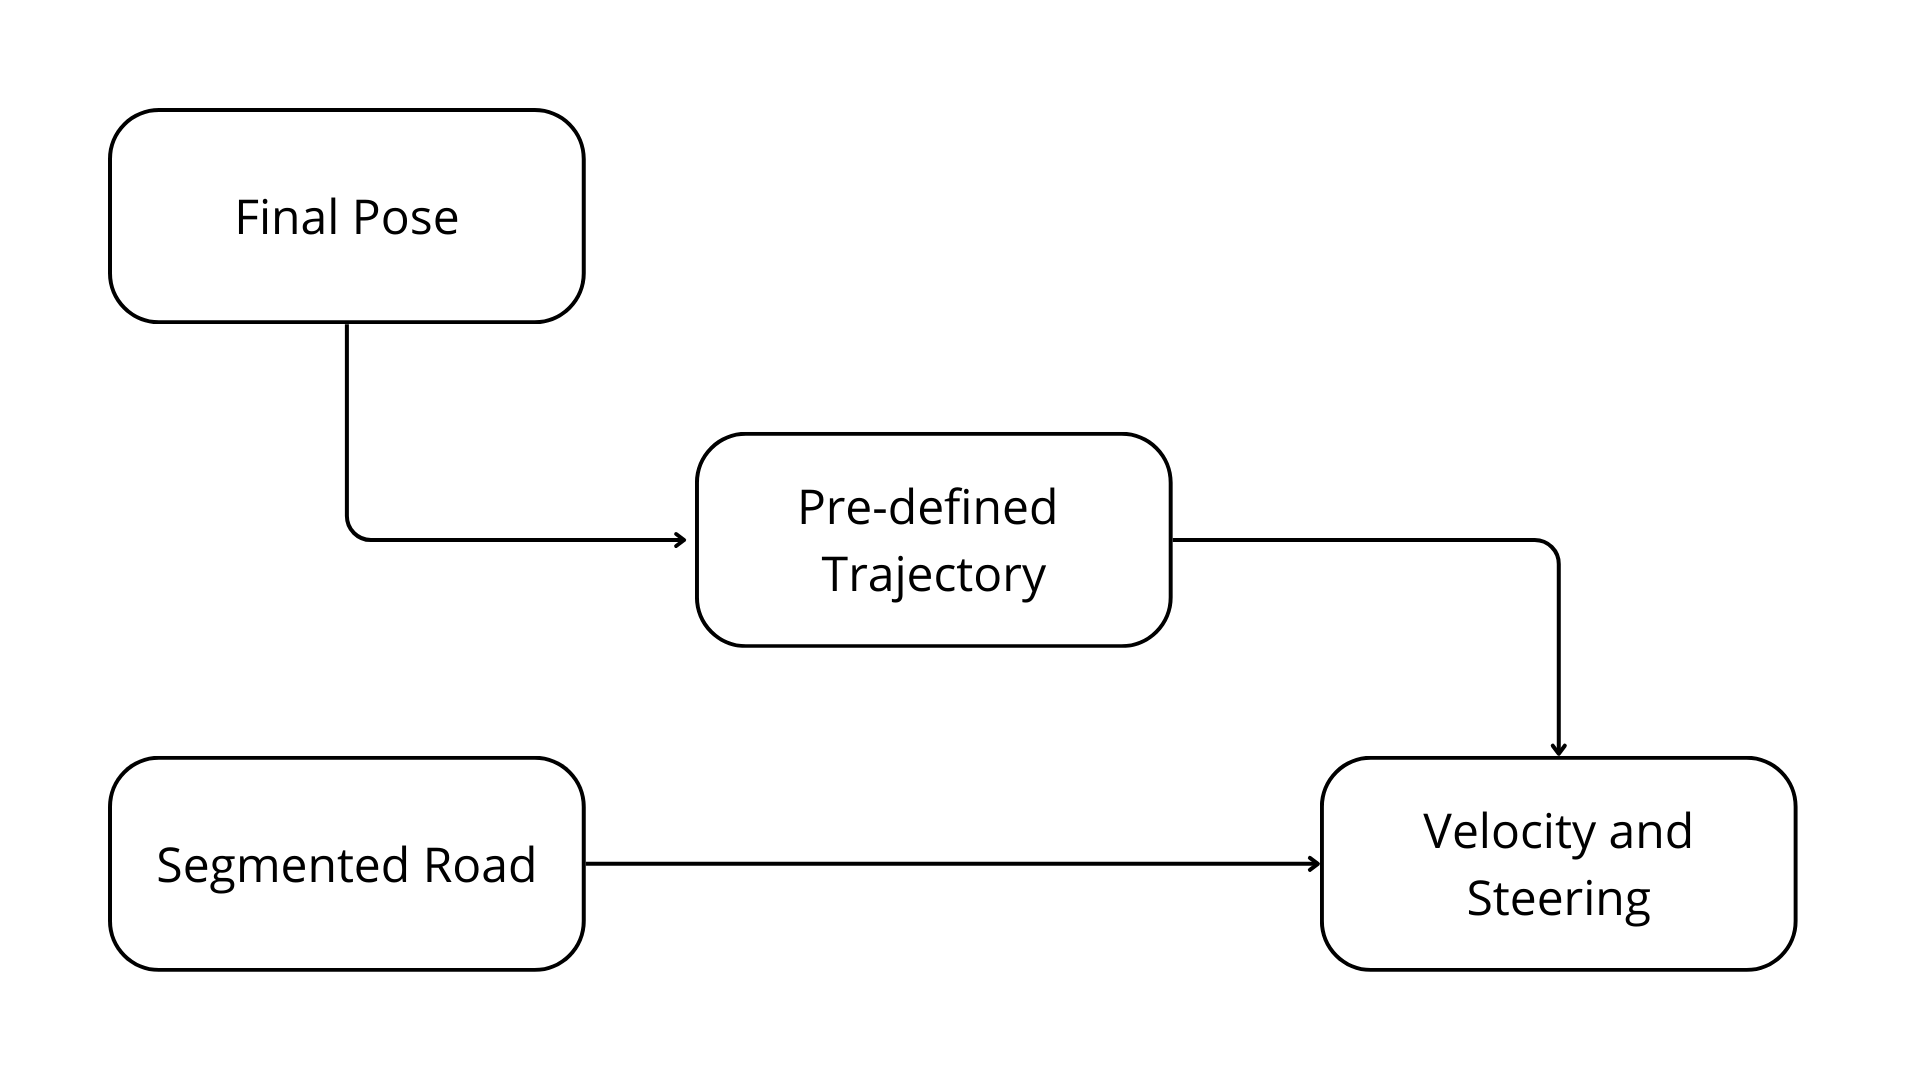
\includegraphics[width=\linewidth]{../konten/nav_sysss.png}
	\caption{Block Diagram Navigation System with Lane Detection and Graph-Based SLAM}
	\label{fig:nav_new_system}
\end{figure} 

The figure \ref{fig:nav_new_system} shows the integration of the navigation system with lane detection and graph-based SLAM. The first step is acquire velocity and steering using Final Pose and Pre-defined Trajectory. This can be done using step below: 

\begin{equation}
	\begin{aligned}
	\theta_{\text{direction}} = \tan^{-1}\left(\frac{y_{\text{wp}} - y_{\text{position}}}{x_{\text{wp}} - x_{\text{position}}}\right) - \theta_{\text{orientation}}
	\label{eq:waypoint_angle}
	\end{aligned}
\end{equation}
Where $x_{\text{wp}}$ and $y_{\text{wp}}$ are the coordinates of the waypoint obtained from the Pre-defined Trajectory, $x_{\text{position}}$ and $y_{\text{position}}$ represent the vehicle's current position, and $\theta_{\text{orientation}}$ is the current orientation of the vehicle. $\theta_{\text{direction}}$ is the heading angle towards the waypoint. With using that angle, we can calculate the target steering angle by using the Bicycle Model as follows:

\begin{equation}
	\begin{aligned}
	\delta_{\text{target}} = \tan^{-1}\left( \frac{2 \cdot L \cdot \sin(\theta_{\text{direction}})}{D_{\text{lookahead}}} \right)
	\label{eq:bicycle_model_full}
	\end{aligned}
\end{equation}
Where $L$ is the distance between the front and rear wheels, and $D_{\text{lookahead}}$ is the lookahead distance. $\delta_{\text{target}}$ is the target steering angle. The target speed is calculated using the following equation:

\begin{equation}
	\begin{aligned}
		v_{\text{target}} &= \min\left(\sqrt{(y_{\text{wp}} - y_{\text{position}})^2 + (y_{\text{wp}} - y_{\text{position}})^2}, \ v_{\text{max}}\right) \\
		\label{eq:bicycle_model_velocity}
	\end{aligned}		
\end{equation}
Where $v_{\text{max}}$ is the maximum speed of the vehicle. The target speed $v_{\text{target}}$ is determined by the distance to the waypoint, ensuring it does not exceed the maximum speed.

\par    
The next step is to calculate the confidence level from segmented lane detection. Before we calculate the confidence level, we need to do ROI (Region of Interest) calculate. First, we create a Circle ROI at center above of the image. The next step is to do bitwise AND between the segmented lane detection and the circle of ROI. After that, we can calculate the normalization of area by divide the final segmented area with maximum ROI. 

\begin{equation}
	\begin{aligned}
	\text{normal} = \frac{\text{area of segmented lane detection}}{\text{area of ROI}}
	\label{eq:confidence_level}
	\end{aligned}
\end{equation}
Where $\text{area of segmented lane detection}$ is the area of the segmented lane detection image, and $\text{area of ROI}$ is the area of the ROI image. The $\text{normal}$ is the normalization value between 0 to 1.
The next step is to calculate the confidence speed based on the normalization value. The confidence speed is calculated by multiplying the maximum speed with the square of the normalization value. The formula is as follows:
\begin{equation}
	\begin{aligned}
		v_{\text{target\_max}} = v_{\text{max}} \cdot \text{normal}^2
	\label{eq:confidence_speed}
	\end{aligned}
\end{equation}
Where $v_{\text{target\_max}}$ is the maximum target speed based on the confidence level, and $v_{\text{max}}$ is the maximum speed of the vehicle. The confidence speed will be used to limit the target speed of the vehicle. To get more smooth transition, the simple low pass filter was used to get the final target speed. The low pass filter is calculated using the following equation:
\begin{equation}
	\begin{aligned}
		v_{\text{target}} = \alpha \cdot v_{\text{target\_max}} + (1 - \alpha) \cdot v_{\text{target}}
	\label{eq:low_pass_filter}
	\end{aligned}
\end{equation}
Where $\alpha$ is the low pass filter coefficient (currently we use 0.055), $v_{\text{target\_max}}$ is the maximum target speed based on the confidence level, and $v_{\text{target}}$ is the previous target speed. The final target speed will be used to control the speed of the vehicle. The use of the low pass filter can prevent the sudden change of the target speed because of image flickering or noise. 

\par    
The last step is to combine it, The target velocity speed from equation \ref{eq:bicycle_model_velocity} will be clipped with the final target speed from equation \ref{eq:low_pass_filter}. The target steering angle from equation \ref{eq:bicycle_model_full} will be used to control the steering of the vehicle. The final target velocity will be sent to the motor driver as a Volt signal and the final target steering angle will be sent to the EPS (Electronic Power Steering) using CAN bus.


\section{Results and Discussion} 
There were several results that we got from this research. The first result is the cm level error (below 1 cm) in robot pose estimation. The second result is the fast lightweight and near accurate lane detection. The third result is the total time to transport the molten aluminum liquid from IST to CMWI. 

\subsection{Robot Pose Estimation} 
There is the result on pose estimation without SLAM. The result is comparing the odometry before and after 500 meters long path. The result is shown in the table \ref{tab:pose_estimation}.
\begin{table}[H]
	\centering
	\caption{Pose Estimation Result without SLAM}
	\label{tab:pose_estimation}
	\begin{tabular}{|c|c|c|c|}
		\hline
		\textbf{Lap-} & \textbf{X (m)} & \textbf{Y (m)} & \textbf{Error (m)} \\ \hline
		1 & 0.26 & 0.37 & 0.45 \\ \hline
		2 & 0.33 & 0.45 & 0.56 \\ \hline
		3 & 0.27 & 0.44 & 0.52 \\ \hline
		4 & 0.15 & 0.35 & 0.38 \\ \hline
		5 & 0.35 & 0.42 & 0.55 \\ \hline
		\multicolumn{3}{|c|}{\textbf{Average Error}} & 0.492 \\ \hline
	\end{tabular}
\end{table}
Where the \textbf{Lap-} is the lap number, \textbf{X (m)} and \textbf{Y (m)} are the position of the Towing in meter after 500 meter moving, and \textbf{Error (m)} is the error of the pose estimation in meter. The error calculated using the ground truth zero condition (x = 0 and y = 0) The average error is 0.492 meters or 49.2 cm. This is not good enough for autonomous navigation, so we need to use SLAM to improve the pose estimation. There is the result on pose estimation using SLAM. The result is shown in the table \ref{tab:pose_estimation_slam}.
\begin{table}[H]
	\centering
	\caption{Pose Estimation Result with SLAM}
	\label{tab:pose_estimation_slam}
	\begin{tabular}{|c|c|c|c|}
		\hline
		\textbf{Lap-} & \textbf{X (m)} & \textbf{Y (m)} & \textbf{Error (m)} \\ \hline
		1 & 0.02 & 0.01 & 0.02 \\ \hline
		2 & 0.00 & 0.03 & 0.03 \\ \hline
		3 & 0.01 & 0.02 & 0.02 \\ \hline
		4 & 0.01 & 0.01 & 0.01 \\ \hline
		5 & 0.02 & 0.04 & 0.04 \\ \hline
		\multicolumn{3}{|c|}{\textbf{Average Error}} & 0.024 \\ \hline
	\end{tabular}
\end{table}
Where the \textbf{Lap-} is the lap number, \textbf{X (m)} and \textbf{Y (m)} are the position of the Towing in meter after 500 meter moving, and \textbf{Error (m)} is the error of the pose estimation in meter. The error calculated using the ground truth zero condition (x = 0 and y = 0) The average error is 0.024 meters or 2.4 cm. This is excellent enough for autonomous navigation, so we can conclude that our architecture in graph based SLAM is working well.

\subsection{Lane Detection}
There are the result from the lane detection using machine learning. The result is shown in the figure \ref{fig:lane_detection_result}.
\begin{figure}[H]
	\centering
	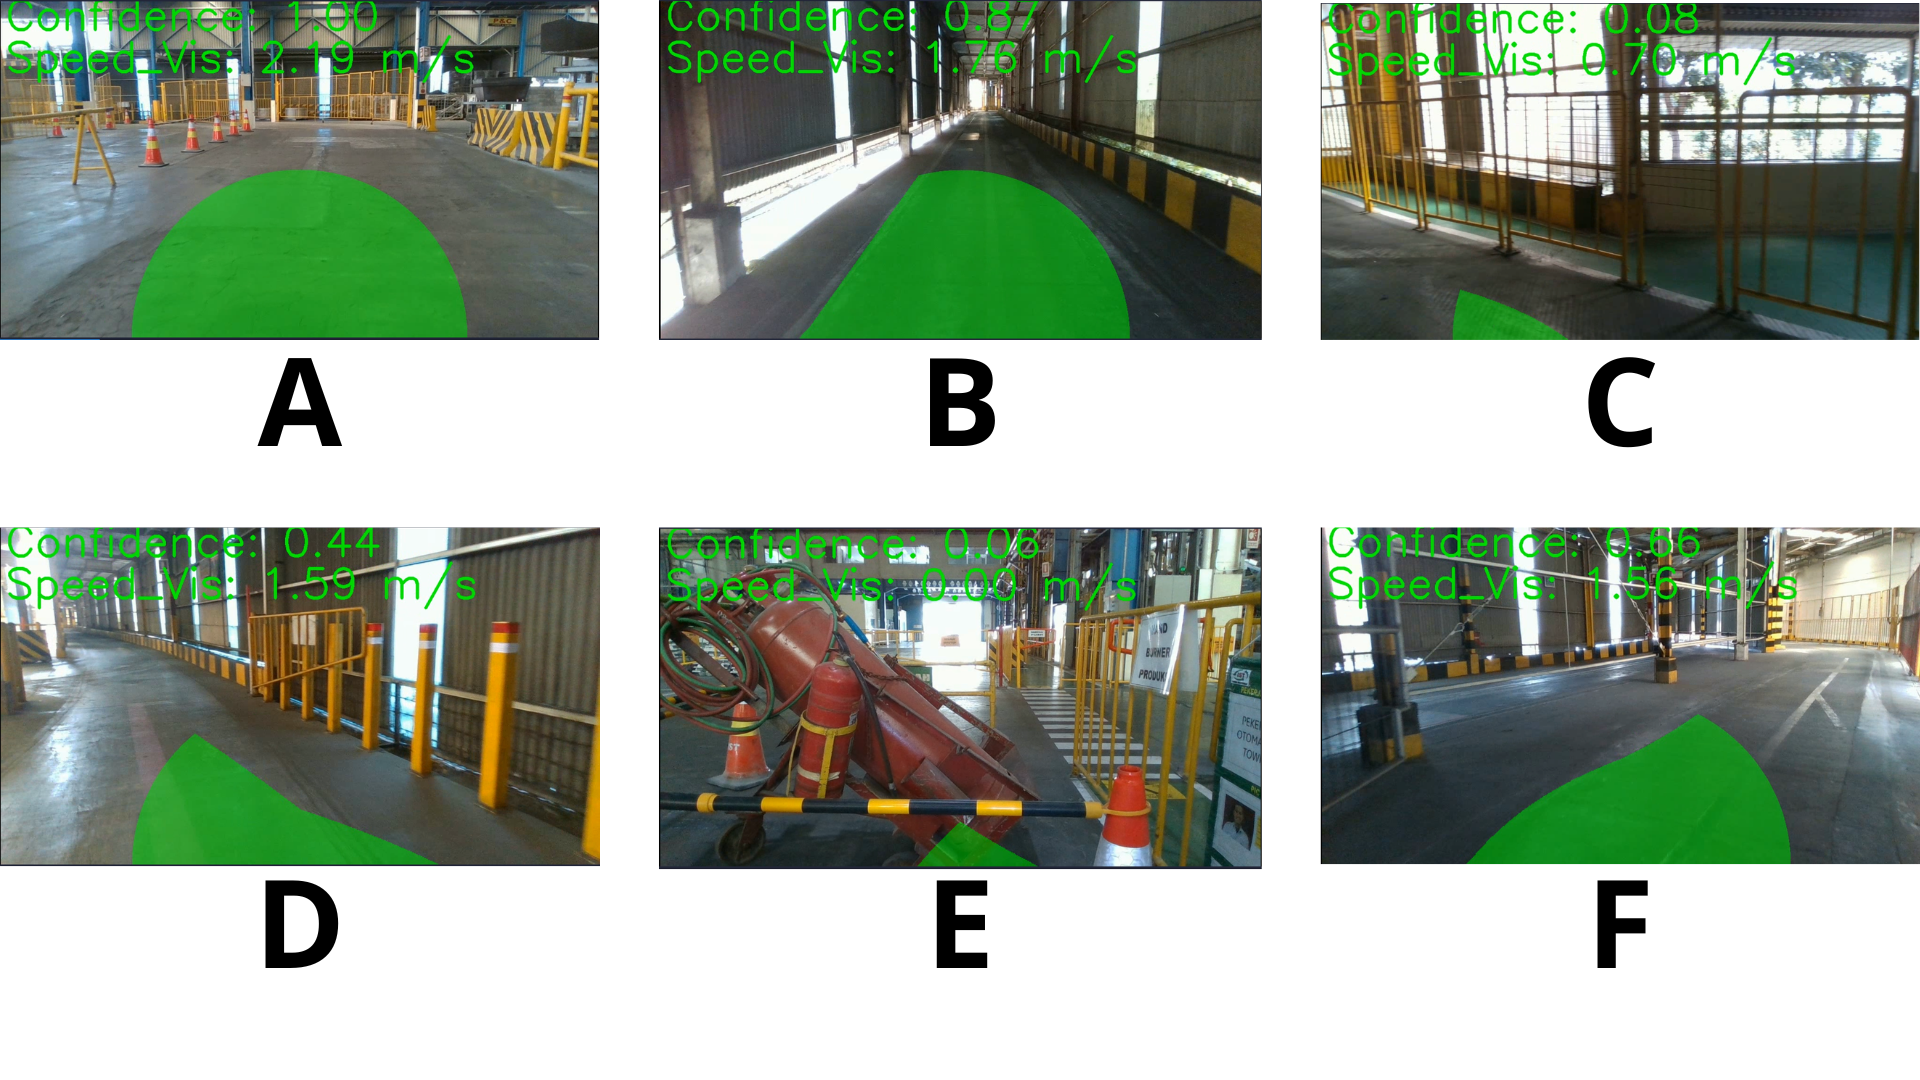
\includegraphics[width=\linewidth]{../konten/bnr_satu.png}
	\caption{Lane Detection Result using Machine Learning}
	\label{fig:lane_detection_result}
\end{figure}
The figure \ref{fig:lane_detection_result} shows the results of lane detection using machine learning. The image A is the condition where Towing at full straight lane, the output velocity is 2.2 meter per seconds. Image B is the condition where Towing is inside narrow straight lane, the output velocity is 1.76 meter per seconds. The image C is the condition where Towing in sharp turn and facing the fences, the output velocity only 0.70 meter per seconds. The image D is the condition where Towing going to turn left with narrow area, the output velocity is 1.59 meter per seconds. The image E is the condition where Towing cannot move because there is an obstacle in the front of Towing, the velocity is 0.00 meter per seconds. The last image F is where Towing goinf turn right with narrow area, the output velocity is 1.56 meter per seconds. 

\par   
Another result is the inference time for one frame of lane detection. The result is shown in the table \ref{tab:lane_detection_inference_time}. 
\begin{table}[H]
	\centering
	\caption{Lane Detection Inference Time}
	\label{tab:lane_detection_inference_time}
	\begin{tabular}{|c|c|}
		\hline
		\textbf{Frame Number} & \textbf{Inference Time (ms)} \\ \hline
		1 & 7.2 \\ \hline
		2 & 7.7 \\ \hline
		3 & 7.8 \\ \hline
		4 & 7.7 \\ \hline
		5 & 7.4 \\ \hline
		6 & 8.0 \\ \hline
		Averate & 7.63 \\ \hline
	\end{tabular}
\end{table}
Table \ref{tab:lane_detection_inference_time} shows the inference time for lane detection using machine learning. The average inference time is 7.63 ms, which is fast enough to run on CPU with low power usage. This is very important for autonomous navigation because the lane detection need to be fast and accurate to detect the lane and obstacles in real-time. That can be obtained by using onnx runtime that can run on CPU \cite{ref_onnx}. 

\subsection{Total Time to Transport the Molten Aluminum Liquid}
There is the result on total time to transport the molten aluminum liquid from IST to CMWI. The result is shown in the table \ref{tab:total_time_transport}.
\begin{table}[H]
	\centering
	\caption{Total Time to Transport the Molten Aluminum Liquid (Autonomous Towing)}
	\label{tab:total_time_transport}
	\begin{tabular}{|c|c|c|}
		\hline
		\textbf{Lap-} & \textbf{Time taken (Minutes)} & \textbf{Molten Sent (Ton)} \\ \hline
		1 & 6.59 & 1.8 \\ \hline
		2 & 7.03 & 1.8 \\ \hline
		3 & 7.06 & 1.8 \\ \hline
		4 & 7.08 & 1.8 \\ \hline
		5 & 7.02 & 1.8 \\ \hline
		6 & 7.03 & 1.8 \\ \hline
		Total & 42.21 & 10.8 \\ \hline
	\end{tabular}
\end{table} 

There is another result on total time to transport the molten aluminum liquid from IST to CMWI with using Manual Drivable Towing. 

\begin{table}[H]
	\centering
	\caption{Total Time to Transport the Molten Aluminum Liquid (Manual Towing)}
	\label{tab:total_time_transport_manual}
	\begin{tabular}{|c|c|c|}
		\hline
		\textbf{Lap-} & \textbf{Time taken (Minutes)} & \textbf{Molten Sent (Ton)} \\ \hline
		1 & 3.29 & 1 \\ \hline
		2 & 4.23 & 1 \\ \hline
		3 & 4.60 & 1 \\ \hline
		4 & 4.56 & 1 \\ \hline
		5 & 3.52 & 1 \\ \hline
		6 & 3.40 & 1 \\ \hline
		Total & 28.20 & 6 \\ \hline
	\end{tabular}
\end{table} 

From table \ref{tab:total_time_transport} and \ref{tab:total_time_transport_manual}, we can see that the total time to transport the molten aluminum liquid from IST to CMWI using Autonomous Towing is 42.21 minutes for 6 laps with total 10.8 tons of molten aluminum liquid sent, while using Manual Towing is 28.20 minutes for 6 laps with total 6 tons of molten aluminum liquid sent. The Autonomous Towing has a longer time because it has to navigate autonomously and detect the lane and obstacles, while the Manual Towing is driven manually by the workers. If we calculate the average time per ton, the Autonomous Towing has 3.91 minutes per ton, while the Manual Towing has 4.70 minutes per ton. This shows that the Autonomous Towing is more efficient in terms of time per ton sent. The 1.8 Tons of molten aluminum liquid can be sent using Autonomous Towing because there will be high risk if the molten sent by manual Towing that drive by the workers.

% \section{Discussion}
% The discussion will be separated into three parts. The first part is the discussion about the architecture of the graph based SLAM. The second part is the discussion about the architecture of the lane detection using machine learning. The last part is the discussion about the integration of the navigation system and safety system. 

% \subsection{Graph Based SLAM Architecture} 
% In our research, we trust more on our hardware odometry because the data from the table \ref{tab:pose_estimation} shows that the error is good enough to be the main odometry for graph based SLAM. We fused the odometry differentially with pose estimated from SLAM. Because of that, we can get realtime update for the final pose of robot in 50 hz control loop.

% \subsection{Lane Detection Architecture}
% The main idea the lane detection is to detect that the Towing is facing the right way or not. Just like a human while driving the car, if there a turn or something terrible in the front of the car like a broken lane or something that block the driver vision, the driver of the car will be slow down the speed of the car. The main reason why the driver slowing down the car is there not enough confidence for the driver to drive the car at high speed. Because of that simple idea, we decide to make the architecture very simple to make the power usage still low. Another reason why we built the architecture very simple is the Autonomous Towing will be always run on same lane so the dataset will be absolute. 

% \par    
% The high speed of the lane detection can be achieved by using an onnx runtime that can run on CPU. We used the pytorch library to train the model and then convert it to onnx format. The onnx runtime can run on CPU with low power usage and low latency. The average inference time based on table \ref{tab:lane_detection_inference_time} is 7.63 ms, which is fast enough for real-time applications. 

% \subsection{Integration of navigation system and safety system} 
% We have an excellent SLAM but we cannot 100\% trust on that because the system is zero fault tolerance. There's the reason why we built another system because if the SLAM fail there still be safety lane detection system that pulls down the velocity to zero to stop the Autonomous Towing. 

\section{Conclusion} 
In this research, we have successfully implemented a full autonomous system on the Towing to transport the molten aluminum liquid from IST to CMWI. The system is robust and can handle the harsh environment in IST. The system can also navigate autonomously using the graph-based SLAM and lane detection using machine learning. The system can also detect the lane and obstacles, and can navigate autonomously to the destination. The result of this research is a cm level error (below 1 cm) in robot pose estimation and a lightweight machine learning model that can run only on CPU with below 10 ms inference time. 

\section{Acknowledgment}
This research is supported by Indonesia Smelting Technology (IST), Manufaktur Robot Industri (MRI), and ITS Robotics. We would like to thank the people who have helped us in this research, especially the team from IST and MRI. We also would like to thank the ITS Robotics team for their support in this research. 


% Menamcement of realsensepilkan daftar pustaka dengan format IEEE
\bibliographystyle{IEEEtranN}
\bibliography{../ubah/pustaka.bib}

% Menyeimbangkan bagian akhir di kedua kolom
% \balance


\end{document}
